
\Aufgabe[e]{Drehungen in $\R^3$}{
Aus der Vorlesung kennen Sie die Matrix einer Drehung im $\R^3$ um eine Koordinatenachse. 
\begin{abc}
\item Geben Sie die Matrix einer Drehung um die $z$-Achse an.\\
Geben Sie au\ss erdem die Matrix einer Drehung um die $x$-Achse an. \\


Um eine allgemeine Drehung im Raum anzugeben, ben\"otigt man drei Drehungen um einzelne
Koordinatenachsen. Diese kann man durch die drei Euler-Winkel $(\phi, \theta, \psi)$ angeben:\\
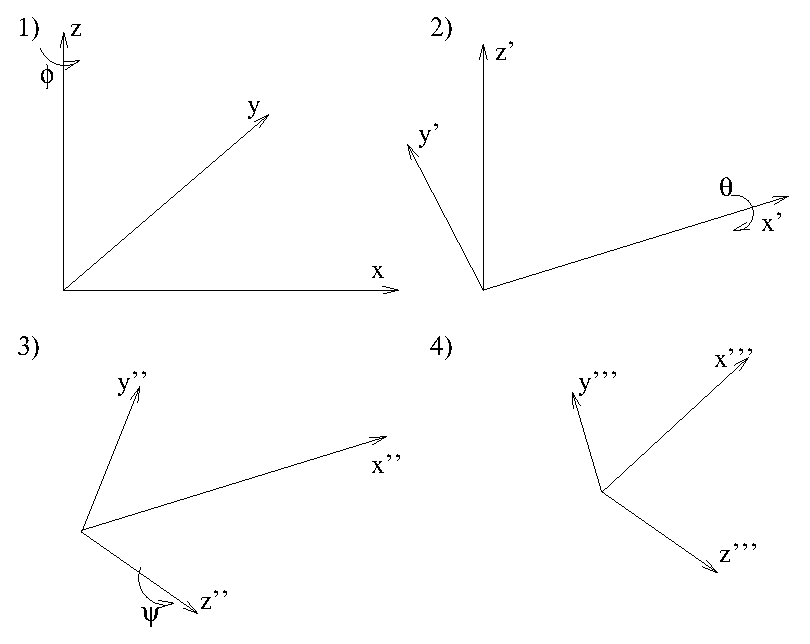
\includegraphics[width=10cm]{../A/Lineare_Algebra/drehung3d.eps}

Das Koordinatensystem wird durch die folgenden drei Drehungen 
$$\Vek f_j: \, \R^3\rightarrow\R^3, \quad j=1,\, 2,\, 3$$
transformiert. \\
Die erste Drehung $\Vek f_1$ (im $\Vek x$-System) ist um den Winkel $\phi$ um die $z$-Achse. Damit
erh\"alt man das $\Vek x'$-Koordinatensystem. \\
Die zweite Drehung $\Vek f_2$ (im $\Vek x'$-System) ist um den Winkel $\theta$ um die $x'$-Achse und
ergibt das $\Vek x''$-System. \\
Die dritte Drehung $\Vek f_3$ schlie\ss lich dreht das Koordinatensystem um den
Winkel $\psi$ um die $z''$-Achse und ergibt das $\Vek x'''$-System. 
\item Geben Sie die Matrizen $\Vek A_j$ der Abbildungen $\Vek f_j$ ($j=1,\, 2,\, 3$) an. 
\item Bestimmen Sie die Matrix $\Vek A$ der Gesamtdrehung $\Vek f_3\circ \Vek f_2\circ \Vek f_1$. 
\item Rechnen Sie nach, dass $\Vek A$ orthogonal ist. Was bedeutet diese Orthogonalit\"at?
\end{abc}

}

\Loesung{
\begin{abc}
\item Die Drehung der $xy$-Ebene um den Winkel $\phi$ hat gem\"aß den Online-\"Ubungen die Matrix 
$$\begin{pmatrix}\cos \phi&\sin\phi\\-\sin\phi&\cos\phi\end{pmatrix}.$$
Da sich die $z$-Koordinate bei dieser Drehung nicht \"andert, ist die Matrix
f\"ur diese Drehung im $\R^3$
$$\Vek M_\phi=\begin{pmatrix}\cos\phi&\sin\phi&0\\-\sin\phi&\cos\phi&0\\0&0&1\end{pmatrix}.$$
Die Drehung der $yz$-Ebene um den Winkel $\theta$ hat, wenn man die
Koordinaten entsprechend vertauscht, die Matrix
$$\Vek M_\theta=\begin{pmatrix}1&0&0\\0&\cos\theta&\sin\theta\\0&-\sin\theta&\cos\theta\end{pmatrix}.$$
\item Die erneute Drehung um die nun anders liegende $z$-Achse um den Winkel
  $\psi$ hat wieder die Gestalt wie in (a):
$$\Vek M_\psi=\begin{pmatrix}\cos\psi&\sin\psi&0\\-\sin\psi&\cos\psi&0\\0&0&1\end{pmatrix}.$$
\item Die Matrix der Gesamtdrehung erh\"alt man schlie\ss lich durch die
Hintereinanderausf\"uhrung dieser drei Drehungen: 
\begin{align*}
&\Vek M_{\phi\theta\psi}\\
=&\Vek M_\psi \Vek M_\theta \Vek M_\phi=\Vek M_\psi \begin{pmatrix}\cos
  \phi&\sin\phi&0\\-\cos\theta\sin\phi&\cos\theta\cos\phi&\sin\theta\\\sin\theta\sin\phi&-\sin\theta\cos\phi&\cos\theta\end{pmatrix}\\
=&\begin{pmatrix}\cos\psi&\sin\psi&0\\-\sin\psi&\cos\psi&0\\0&0&1\end{pmatrix}\begin{pmatrix}\cos
  \phi&\sin\phi&0\\-\cos\theta\sin\phi&\cos\theta\cos\phi&\sin\theta\\\sin\theta\sin\phi&-\sin\theta\cos\phi&\cos\theta\end{pmatrix}\\
=&\begin{pmatrix}\cos\psi\cos\phi-\sin\psi\cos\theta\sin\phi&\cos\psi\sin\phi+\sin\psi\cos\theta\cos\phi&\sin\psi\sin\theta\\-\sin\psi\cos\phi-\cos\psi\cos\theta\sin\phi&-\sin\psi\sin\phi+\cos\psi\cos\theta\cos\phi&\cos\psi\sin\theta\\\sin\theta\sin\phi&-\sin\theta\cos\phi&\cos\theta\end{pmatrix} 
\end{align*}

\item Um zu zeigen, dass $\Vek M_{\phi\theta\psi}$ orthogonal ist, rechnen wir 
 $\Vek M_{\phi\theta\psi}^*\Vek M_{\phi\theta\psi}=\Vek E$ nach: 
\begin{align*}
&\Vek M_{\phi\theta\psi}^*\Vek M_{\phi\theta\psi}\\
=&(\Vek M_\psi\Vek M_\theta \Vek M_\phi)^*\Vek M_\psi\Vek M_\theta\Vek M_\phi=\Vek M_\phi^*\Vek
M_\theta^* \Vek M_\psi^* \Vek M_\psi\Vek M_\theta\Vek M_\phi\\
=&\Vek M_\phi^* \Vek
M_\theta^* \begin{pmatrix} \cos\psi&-\sin\psi&0\\\sin\psi&\cos\psi&0\\0&0&1\end{pmatrix}\begin{pmatrix} \cos\psi&\sin\psi&0\\-\sin\psi&\cos\psi&0\\0&0&1\end{pmatrix}\Vek
M_\theta\Vek M_\phi\\
=&\Vek M_\phi^* \Vek
M_\theta^* \begin{pmatrix} \cos^2\psi+\sin^2\psi&0&0\\0&\sin^2\psi+\cos^2\psi&0\\0&0&1\end{pmatrix} \Vek
M_\theta\Vek M_\phi\\
=& \Vek
M_\phi^*\begin{pmatrix}1&0&0\\0&\cos\theta&-\sin\theta\\0&\sin\theta&\cos\theta\end{pmatrix} \Vek
E \begin{pmatrix}1&0&0\\0&\cos\theta&\sin\theta\\0&-\sin\theta&\cos\theta\end{pmatrix} \Vek
M_\phi\\
=&\Vek M_\phi^* \Vek M_\phi = \Vek E\quad \text{(analog zur Berechnung von $\Vek M_\psi^*\Vek M_\psi$)}
\end{align*}
Die Orthogonalit\"at der Drehmatrix $\Vek M_{\phi\theta\psi}$ hat zur Folge, dass der Wert des Skalarproduktes  zweier Vektoren
$\Vek u,\, \Vek v\in\R^3$ erhalten bleibt, nachdem man sie gedreht hat: 
\begin{align*}
\skalar{\Vek M_{\phi\theta\psi} \Vek u,\, \Vek M_{\phi\theta\psi} \Vek v} = & \bigl( \Vek
M_{\phi\theta\psi}\Vek v\bigr)^*\Vek M_{\phi\theta\psi} \Vek u\\
=& \Vek v^* \Vek M_{\phi\theta\psi}^* \Vek M_{\phi\theta\psi} \Vek u=\Vek v^* \Vek E \Vek u
= \skalar{\Vek u,\Vek v}.
\end{align*}
Insbesondere werden deswegen L\"angen von Vektoren und Winkel zwischen Vektoren durch die Drehung
des Koordinatensystems nicht ver\"andert. 
\end{abc}

}

%\ErgebnisC{AufglinalgEulrWnkl001}
%{
%}
